\section{CP Asymmetry Study}

The selected candidates can be separated into charge-conjugate samples using the
total charge of the three daughter tracks,
\begin{equation}
  Q_{\mathrm{tot}} = Q(H_1) + Q(H_2) + Q(H_3).
\end{equation}
Candidates with $Q_{\mathrm{tot}}=+1$ are classified as \Bplus{} candidates,
while candidates with $Q_{\mathrm{tot}}=-1$ are classified as \Bminus{}
candidates. This assignment uses only reconstructed track-charge information
and is therefore a natural first step toward a charge-asymmetry study in a
three-charged-hadron final state.

\subsection{Charge-separated invariant-mass fits}

Rather than counting candidates in a fixed signal window, the updated
asymmetry extraction fits the \Bplus{} and \Bminus{} invariant-mass spectra
separately. Each charge sample is fitted in the range
$5000 < m(hhh) < 5600~\mevcc$ with a common-mean double-Gaussian signal model
and a finite-range exponential background model. The double-Gaussian signal
shape provides a narrow core plus a broader resolution component, which is a
more realistic detector-level description than a single Gaussian.

The fitted spectra are shown in Fig.~\ref{fig:charge_fit_plus} and
Fig.~\ref{fig:charge_fit_minus}. The fits converge for both charge categories
and give acceptable goodness-of-fit values, with
$\chi^2/\mathrm{ndof}=1.42$ for the \Bplus{} sample and
$\chi^2/\mathrm{ndof}=0.79$ for the \Bminus{} sample. The fitted signal yields
are
\begin{align}
  N(\Bplus) &= 694.4 \pm 27.2, \\
  N(\Bminus) &= 640.0 \pm 25.8,
\end{align}
where the uncertainties are the statistical yield uncertainties returned by
the binned mass fits.

\begin{figure}[H]
  \centering
  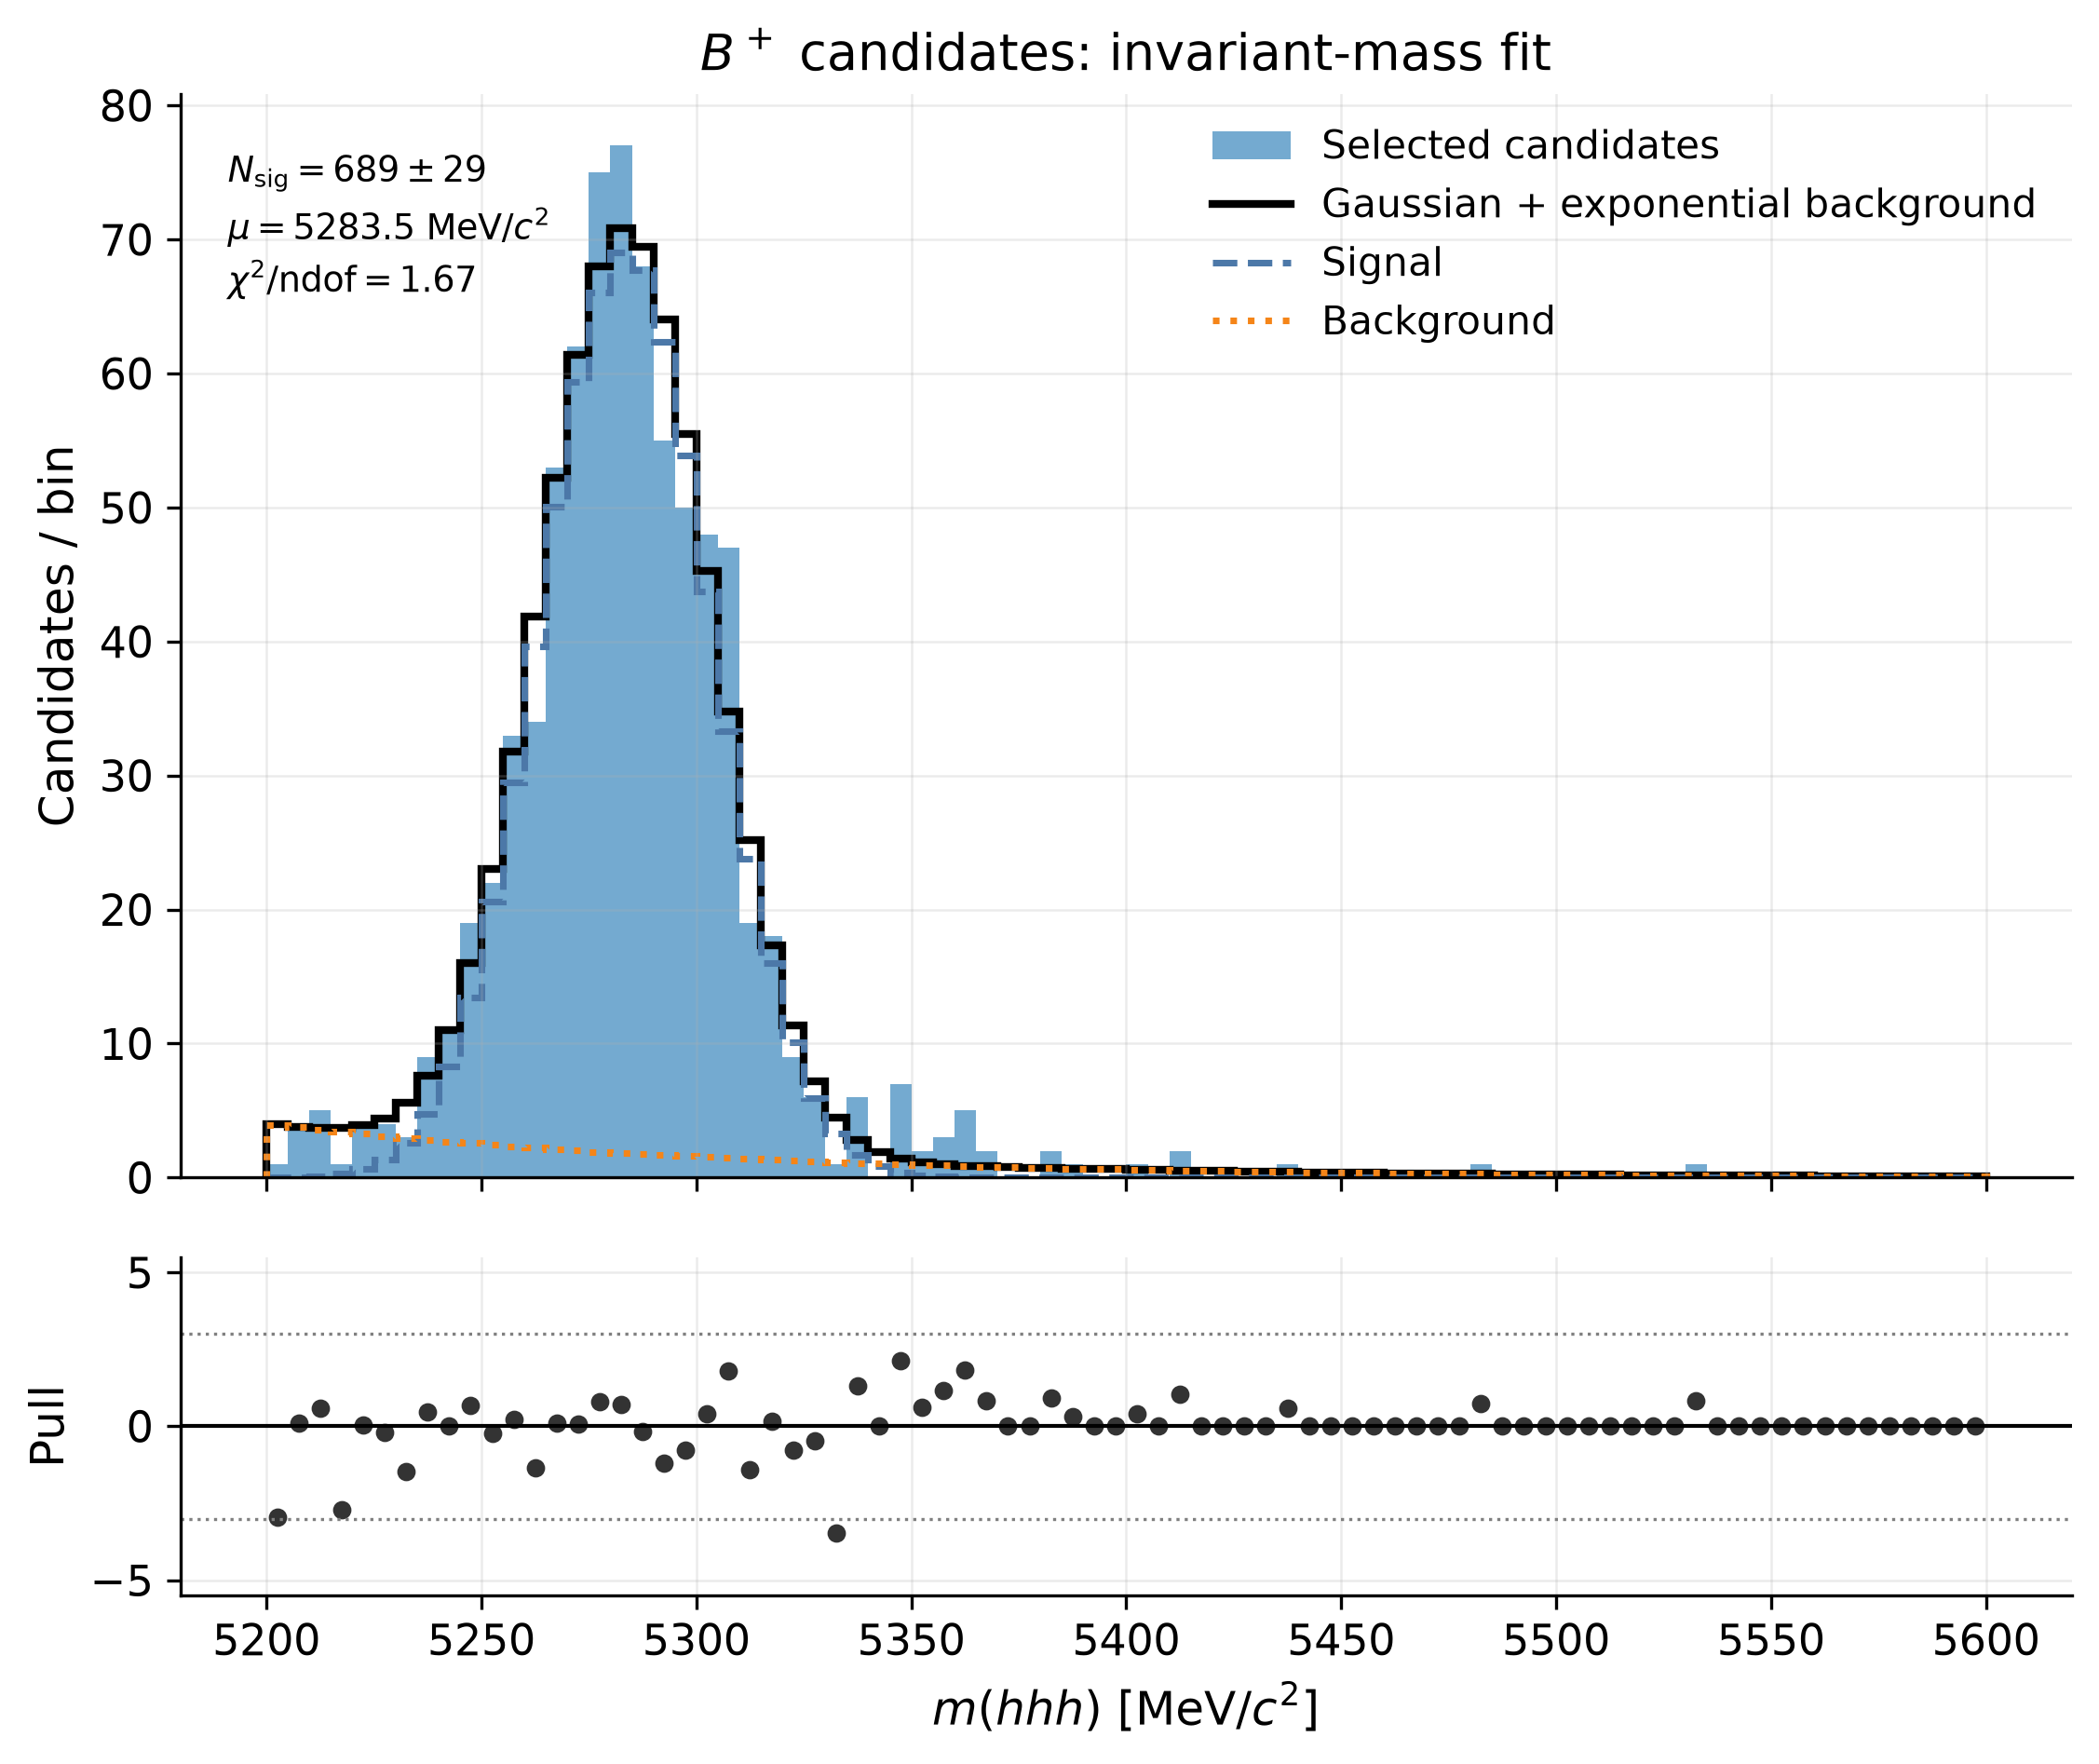
\includegraphics[width=0.82\textwidth]{B_plus_fit_plot.png}
  \caption{Charge-separated invariant-mass fit for the \Bplus{} candidate sample.}
  \label{fig:charge_fit_plus}
\end{figure}

\begin{figure}[H]
  \centering
  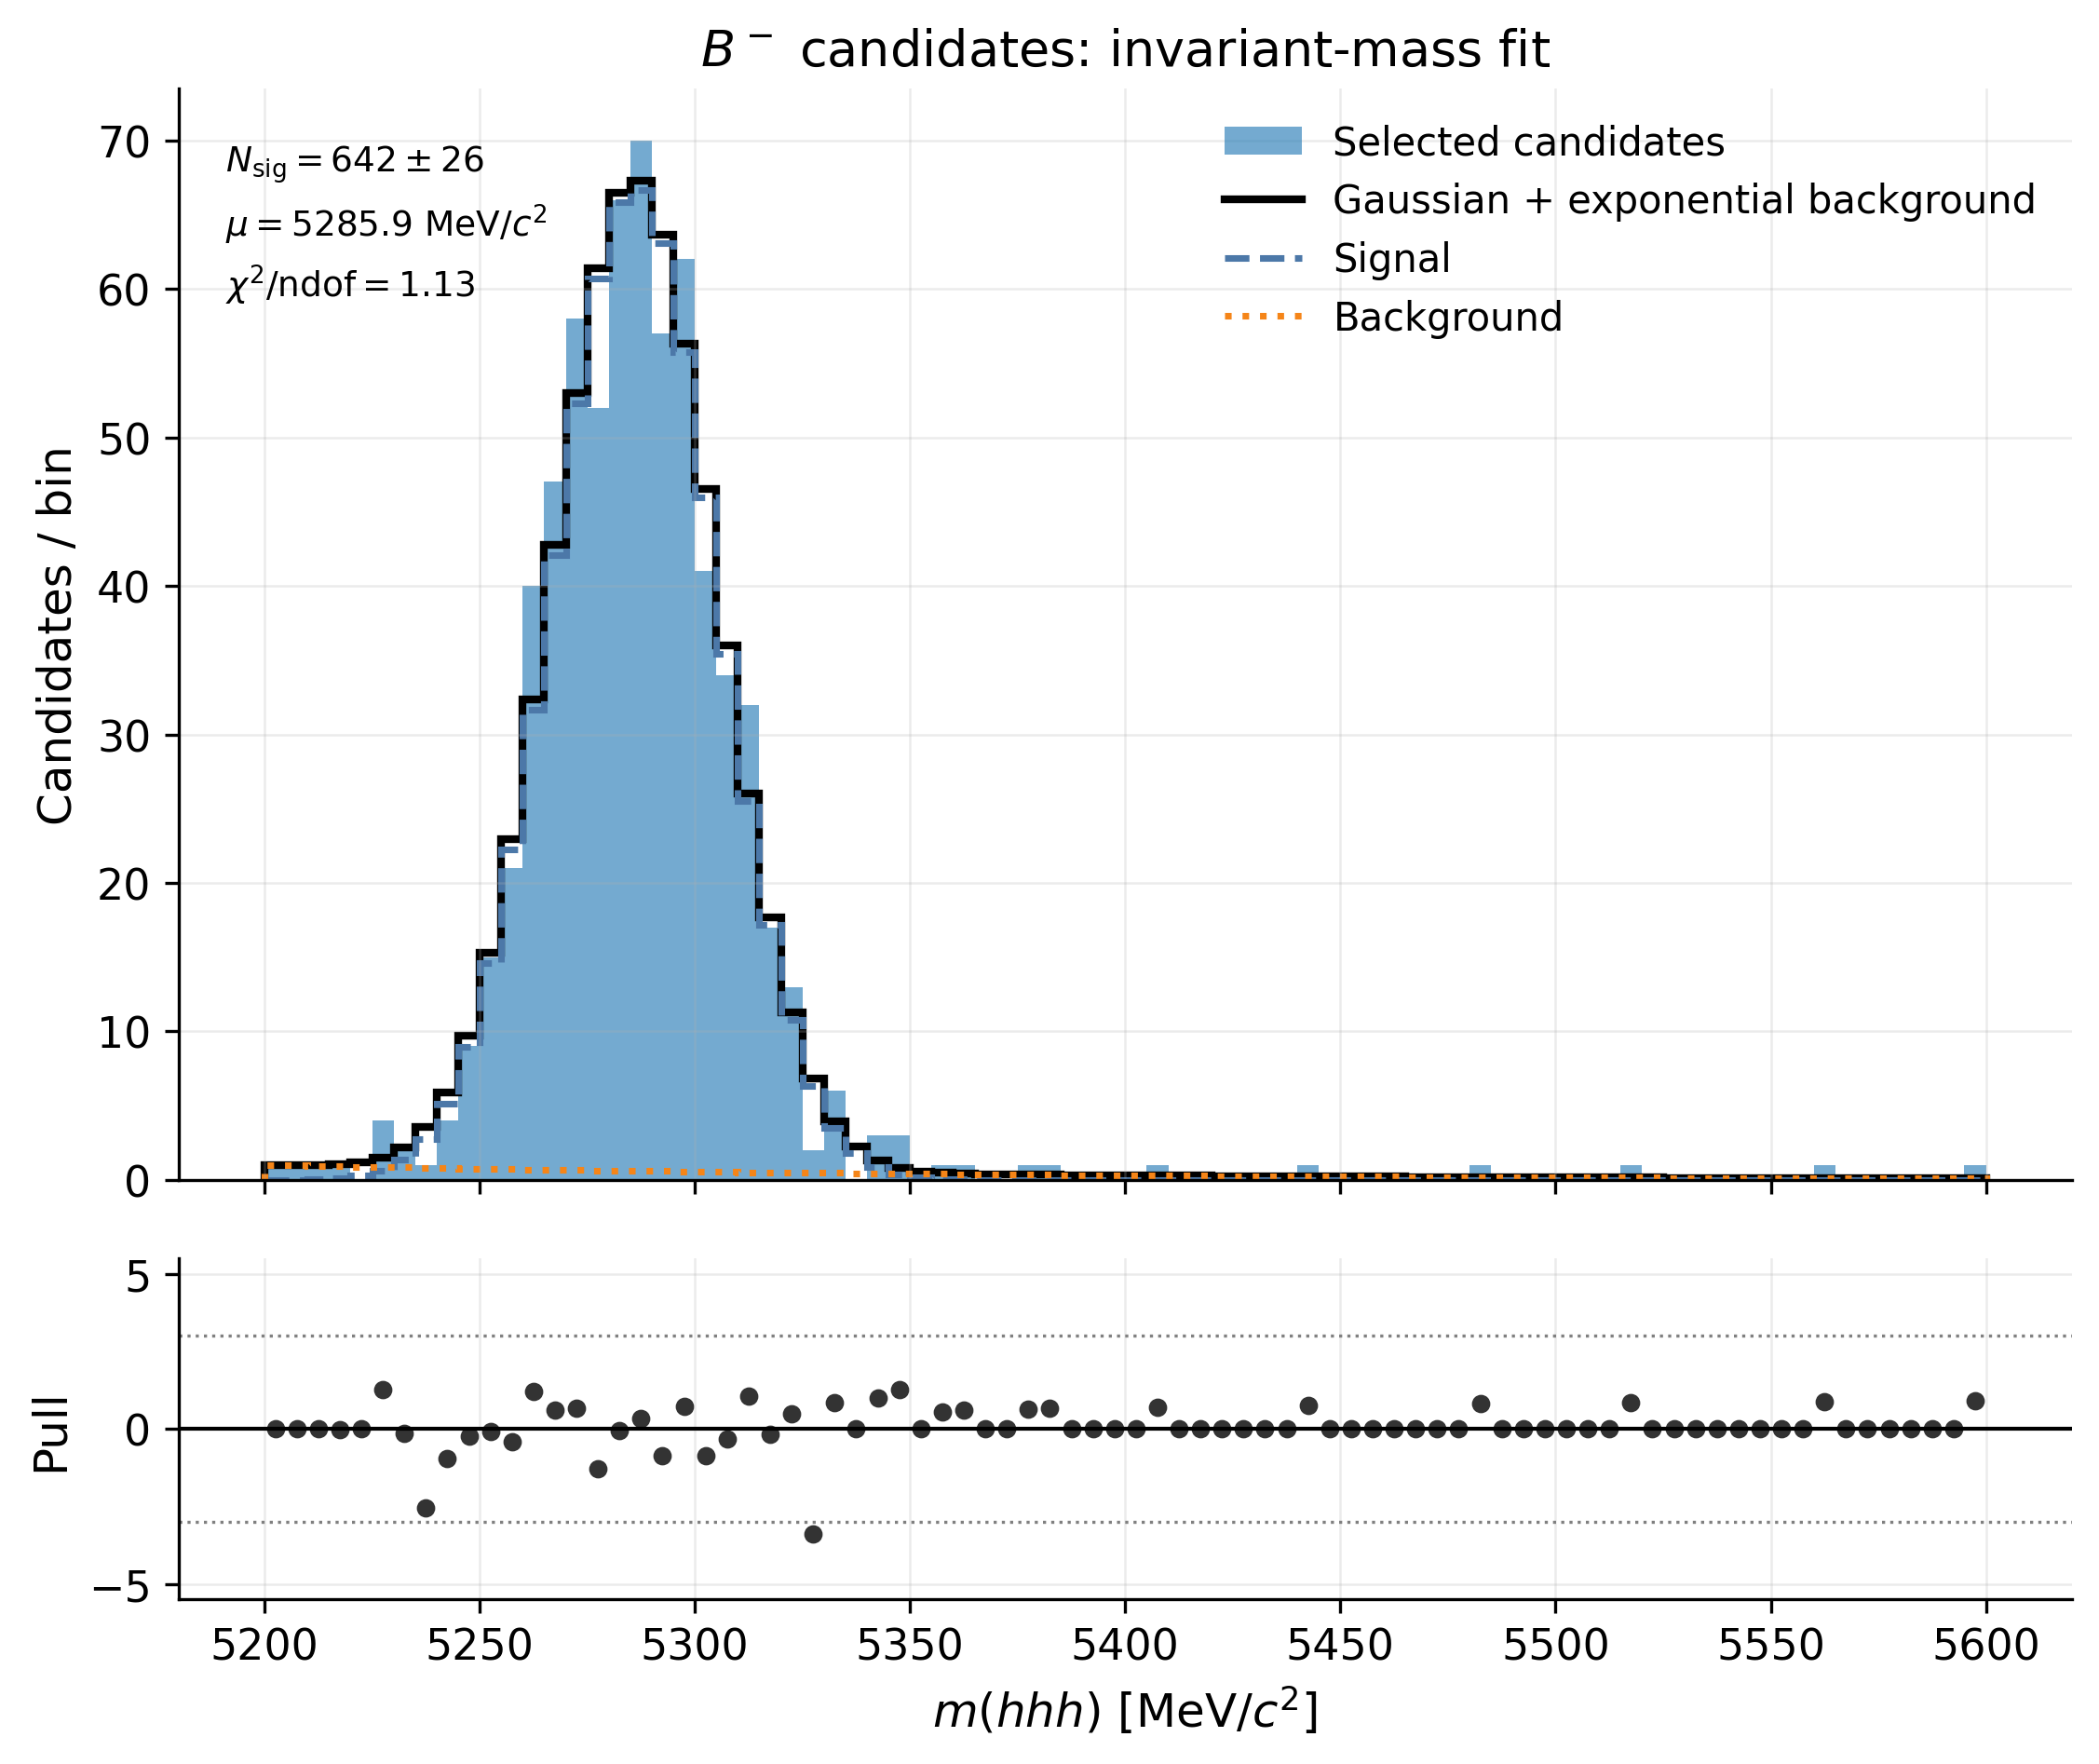
\includegraphics[width=0.82\textwidth]{B_minus_fit_plot.png}
  \caption{Charge-separated invariant-mass fit for the \Bminus{} candidate sample.}
  \label{fig:charge_fit_minus}
\end{figure}

\subsection{Raw asymmetry extraction}

The fitted signal yields are used to construct the raw asymmetry
\begin{equation}
  A_{\mathrm{raw}} =
  \frac{N(\Bminus)-N(\Bplus)}
       {N(\Bminus)+N(\Bplus)} .
  \label{eq:raw_asymmetry_fit}
\end{equation}
Propagating the independent fitted-yield uncertainties gives
\begin{equation}
  A_{\mathrm{raw}} = -0.0408 \pm 0.0281~\mathrm{(stat.)}.
\end{equation}
After including the systematic variations described below, the result is
reported as
\begin{equation}
  A_{\mathrm{raw}} =
  -0.0408 \pm 0.0281~\mathrm{(stat.)}
  \pm 0.0433~\mathrm{(syst.)}.
  \label{eq:raw_asymmetry_result}
\end{equation}

This is a raw asymmetry, not a physical CP-asymmetry measurement. It still
contains detector-induced charge asymmetries, possible \Bplus{}/\Bminus{}
production asymmetries, trigger and reconstruction effects, residual
background-model dependence, and selection-induced charge biases. A complete
measurement would require detector calibration, magnet-polarity combination,
background control, efficiency corrections, and a more complete systematic
uncertainty programme. The value in Eq.~\ref{eq:raw_asymmetry_result} should
therefore be interpreted as a diagnostic of the analysis workflow rather than
as evidence for CP violation.

\subsection{Toy-MC validation}

The statistical machinery was validated with pseudo-experiments generated from
the nominal charge-separated fitted model. In each toy experiment, \Bplus{} and
\Bminus{} mass spectra were generated with the injected fitted yields and then
refitted with the same double-Gaussian plus exponential model used in the data
fit. The toy study checks whether the fitting and uncertainty propagation
recover the injected raw asymmetry when the fit model is correct.

A 100-toy validation with fixed random seed produced 99 toys suitable for pull
studies and no fit failures. For the valid toys, the mean raw-asymmetry pull
was $-0.049$ and the pull width was $1.052$, compatible with the expected
standard normal behaviour for this sample size. The fitted bias was
$-0.0025$, well below the typical fitted statistical uncertainty of about
$0.029$. These results indicate that the nominal statistical extraction is
well behaved on pseudo-data generated from the fitted model. This validation is
not a detector-level systematic study.

\subsection{Systematic uncertainties}

Two first systematic categories are evaluated for the raw asymmetry: the choice
of mass-fit model and the choice of invariant-mass fit range. In both cases,
alternative fits are accepted only if the \Bplus{} and \Bminus{} fits converge,
the fitted yields and yield uncertainties are positive, and the
$\chi^2/\mathrm{ndof}$ values remain below 2.5 for both charge-separated mass
spectra.

The fit-model study compares the nominal double-Gaussian plus exponential model
with an accepted double-Gaussian plus linear-background alternative. A
single-Gaussian plus exponential model is also retained as a stress test, but
it is not used to assign the systematic uncertainty because it does not provide
an acceptable description of the \Bminus{} spectrum. The accepted
linear-background variation shifts the raw asymmetry by $0.0255$, which is
taken as the fit-model systematic uncertainty.

\begin{figure}[H]
  \centering
  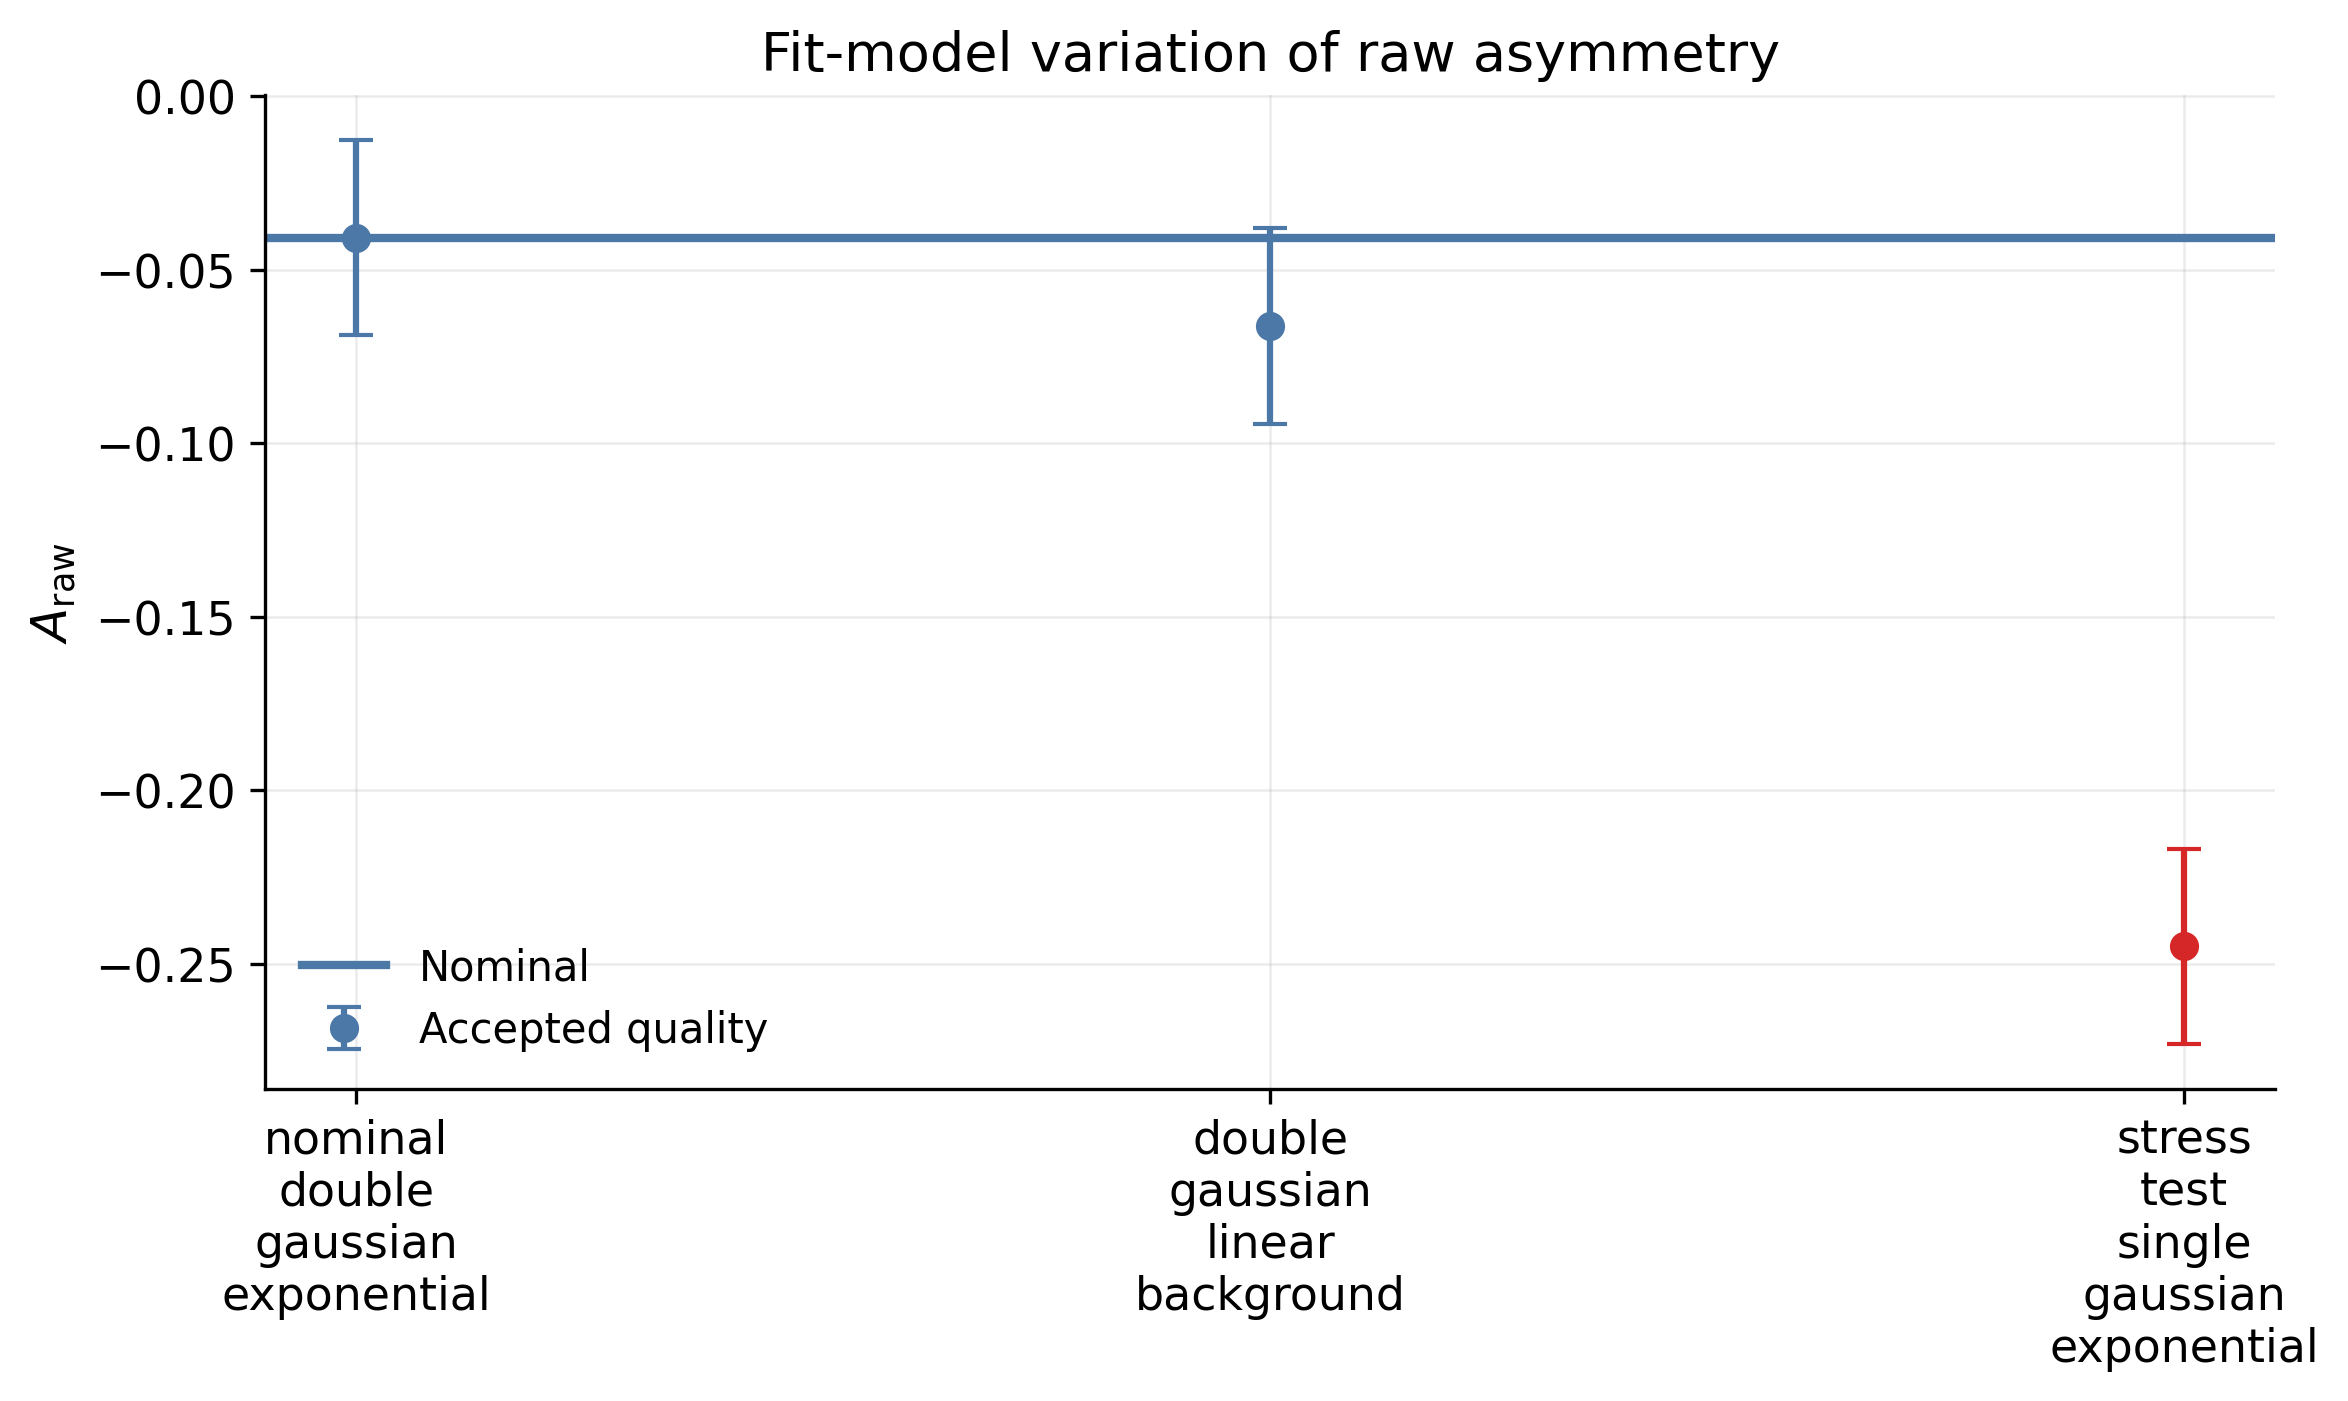
\includegraphics[width=0.82\textwidth]{fit_model_variations.png}
  \caption{Raw asymmetry obtained with different charge-separated mass-fit models. Rejected stress-test variations are shown for comparison but are not used in the systematic assignment.}
  \label{fig:fit_model_systematic}
\end{figure}

The fit-range study repeats the nominal double-Gaussian plus exponential fits
for narrower and wider mass intervals. These variations test the sensitivity
to the amount of sideband information included in the background constraint.
All tested fit-range variations pass the quality requirements. The largest
accepted shift is $0.0350$, obtained from the wider high-mass range
$5000 < m(hhh) < 5700~\mevcc$, and is assigned as the fit-range systematic
uncertainty.

\begin{figure}[H]
  \centering
  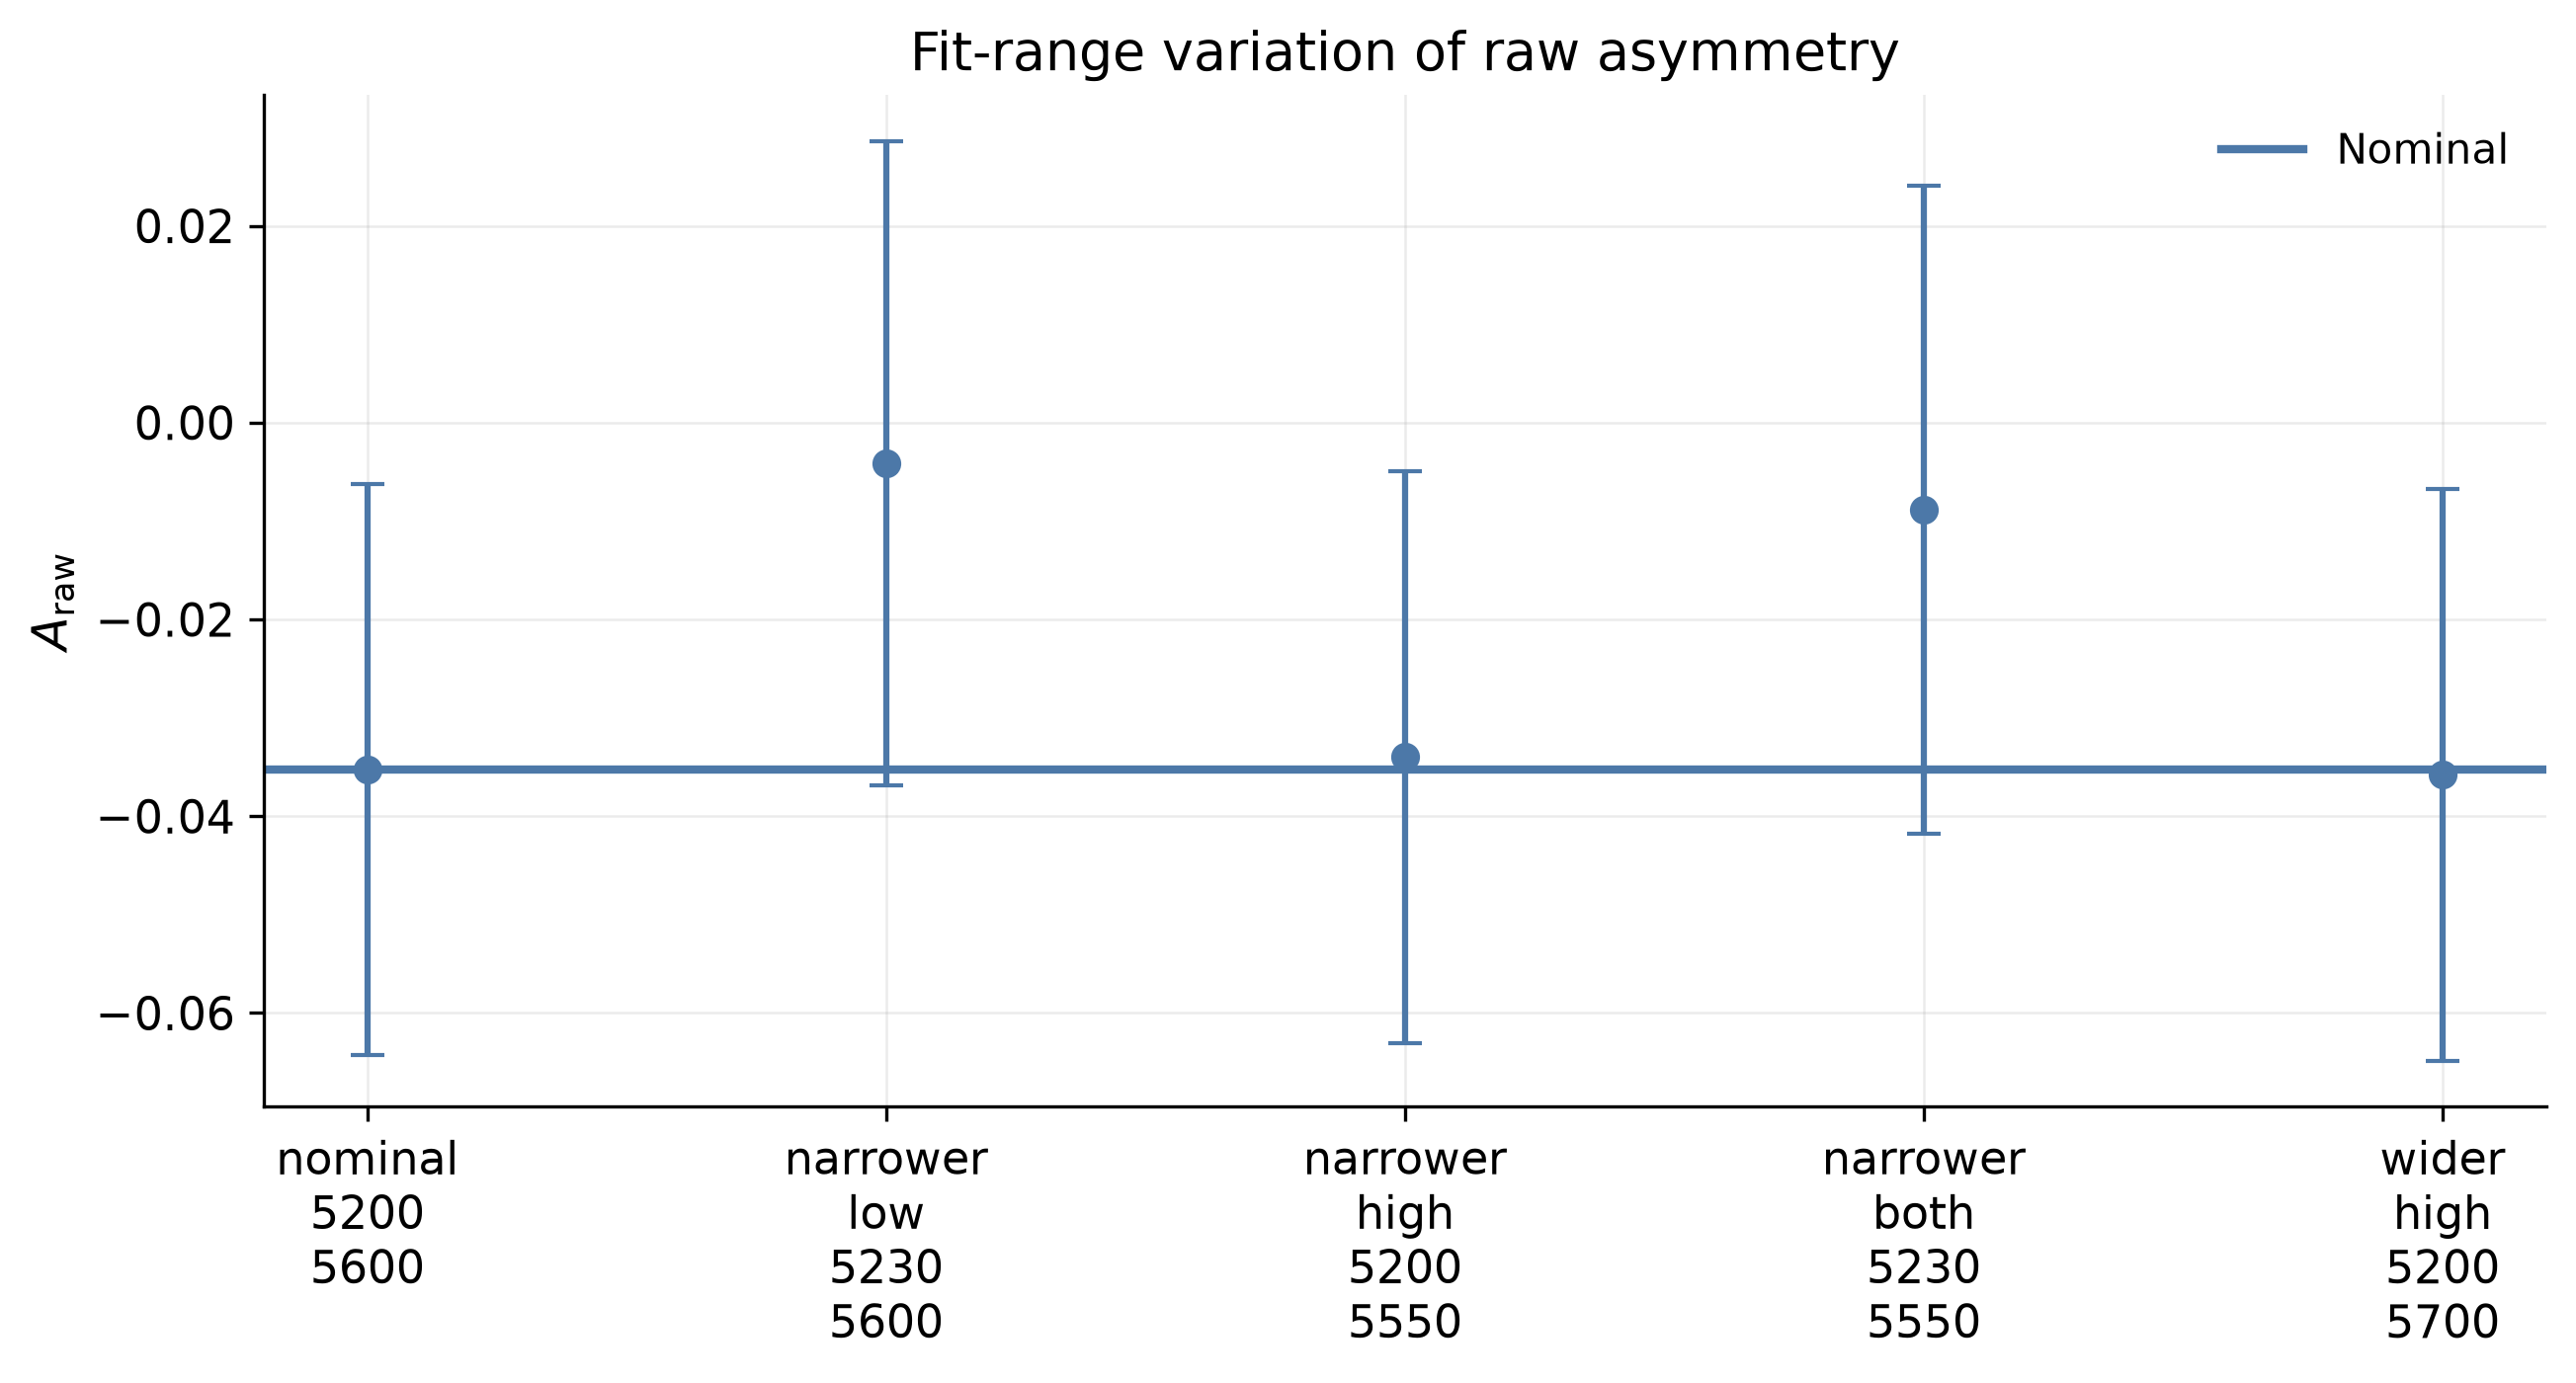
\includegraphics[width=0.82\textwidth]{fit_range_variations.png}
  \caption{Raw asymmetry obtained for alternative invariant-mass fit ranges using the nominal signal and background model.}
  \label{fig:fit_range_systematic}
\end{figure}

Table~\ref{tab:raw_asymmetry_uncertainties} summarizes the uncertainty
components. The total systematic uncertainty is obtained by adding the
fit-model and fit-range components in quadrature. The total uncertainty,
including statistics, is $0.0516$.

\begin{table}[H]
  \centering
  \caption{Uncertainty components for the fitted raw asymmetry.}
  \label{tab:raw_asymmetry_uncertainties}
  \begin{tabular}{lc}
    \toprule
    Source & Uncertainty on $A_{\mathrm{raw}}$ \\
    \midrule
    Statistical & 0.0281 \\
    Fit-model systematic & 0.0255 \\
    Fit-range systematic & 0.0350 \\
    Total systematic & 0.0433 \\
    \bottomrule
  \end{tabular}
\end{table}

\begin{figure}[H]
  \centering
  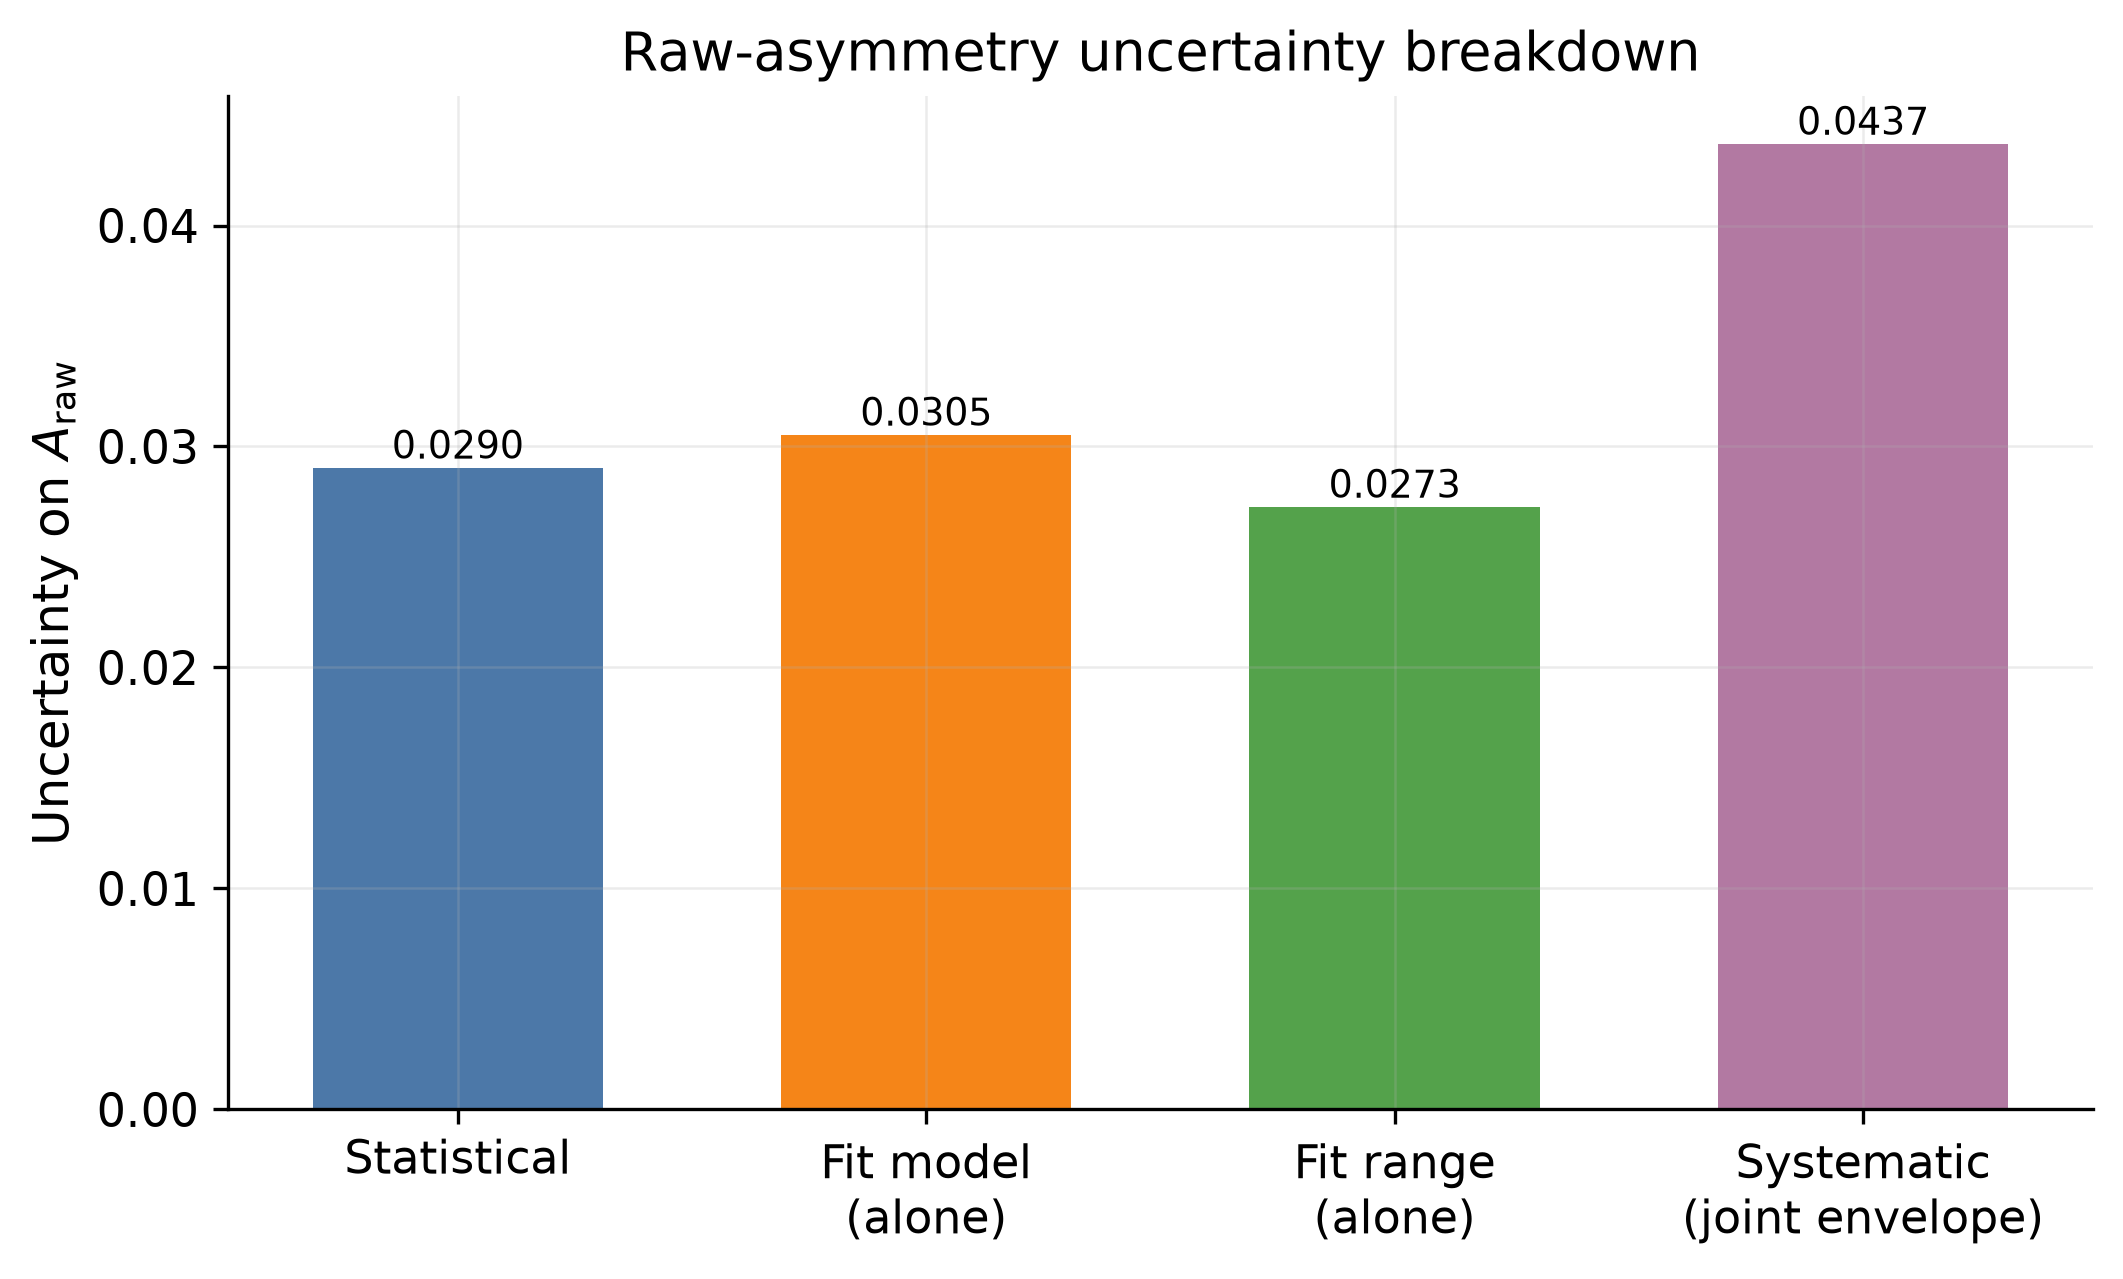
\includegraphics[width=0.72\textwidth]{systematic_breakdown.png}
  \caption{Breakdown of the statistical uncertainty, individual systematic components, and total systematic uncertainty on the raw asymmetry.}
  \label{fig:systematic_breakdown}
\end{figure}

The dominant systematic contribution in this first study comes from the fit
range, followed by the background-model variation. These studies probe only a
limited set of analysis choices. Additional signal-shape variations, broader
background-shape alternatives, magnet-polarity comparisons, and
detector-efficiency corrections would be required before interpreting the raw
asymmetry as a corrected CP observable.

\clearpage
